\documentclass[12pt, a4paper]{article}
\usepackage[swedish, english]{babel}
\usepackage[utf8]{inputenc}
\usepackage{amsmath}
%\usepackage{amsthm}
\usepackage{amssymb}
\usepackage{lmodern}
\usepackage[T1]{fontenc}
\usepackage{units}
\usepackage{icomma}
\usepackage{color}
\usepackage{float}
%\usepackage{amsfonts} %not in use
\usepackage{cancel}
\usepackage{graphicx}
\usepackage{bbm}
\usepackage{enumerate}
\usepackage{textcomp}
\usepackage{enumitem}
\usepackage{alltt}
\usepackage{amsthm}
\usepackage{datetime}
\usepackage[top=2in, bottom=1.5in, left=1.2in, right=1.2in]{geometry}
\usepackage[font=small,labelfont=bf]{caption}
\usepackage{hyperref} \hypersetup{ colorlinks=true,linktoc=all, linkcolor=blue}

\usepackage{bm}
\usepackage{fancyhdr}
\pagestyle{fancy} 
\fancyhead{} % clear all header fields
\fancyhead[L]{\normalfont\scshape\small \selectfont Edvin Listo Zec}
\fancyhead[R]{\normalfont\scshape\small \selectfont Theorems\&Proofs}
\newcommand{\N}{\ensuremath{\mathbbm{N}}}
\newcommand{\Z}{\ensuremath{\mathbbm{Z}}}
\newcommand{\Q}{\ensuremath{\mathbbm{Q}}}
\newcommand{\R}{\ensuremath{\mathbbm{R}}}
\newcommand{\C}{\ensuremath{\mathbbm{C}}}
\newcommand{\rd}{\ensuremath{\mathrm{d}}}
\newcommand{\id}{\ensuremath{\,\rd}}
% % command below makes a bold x, v and a
% % used for vector notation.
\newcommand{\xb}{\ensuremath{\mathbf{x}}}
\newcommand{\ab}{\ensuremath{\mathbf{a}}}
\newcommand{\vb}{\ensuremath{\mathbf{v}}}

%% http://en.wikibooks.org/wiki/LaTeX/Advanced_Mathematics

%% //ROBIN: ADDED CODE BELOW 2014-12-08, TO SUPPORT FOR MATLAB CODE
%% TO INPUT MATLAB CODE INPUT: \lstinputlisting[language=matlab]{source_filename.m}
\usepackage{listings}
\definecolor{mygreen}{rgb}{0,0.6,0}
\definecolor{mygray}{rgb}{0.5,0.5,0.5}
\definecolor{mymauve}{rgb}{0.58,0,0.82}

\lstset{ %
  backgroundcolor=\color{white},   % choose the background color; you must add \usepackage{color} or \usepackage{xcolor}
  basicstyle=\footnotesize,        % the size of the fonts that are used for the code
  breakatwhitespace=false,         % sets if automatic breaks should only happen at whitespace
  breaklines=true,                 % sets automatic line breaking
  captionpos=b,                    % sets the caption-position to bottom
  commentstyle=\color{mygreen},    % comment style
  deletekeywords={...},            % if you want to delete keywords from the given language
  escapeinside={\%*}{*)},          % if you want to add LaTeX within your code
  extendedchars=true,              % lets you use non-ASCII characters; for 8-bits encodings only, does not work with UTF-8
  frame=single,                    % adds a frame around the code
  keepspaces=true,                 % keeps spaces in text, useful for keeping indentation of code (possibly needs columns=flexible)
  keywordstyle=\color{blue},       % keyword style
  language=Octave,                 % the language of the code
  morekeywords={*,...},            % if you want to add more keywords to the set
  numbers=left,                    % where to put the line-numbers; possible values are (none, left, right)
  numbersep=5pt,                   % how far the line-numbers are from the code
  numberstyle=\tiny\color{mygray}, % the style that is used for the line-numbers
  rulecolor=\color{black},         % if not set, the frame-color may be changed on line-breaks within not-black text (e.g. comments (green here))
  showspaces=false,                % show spaces everywhere adding particular underscores; it overrides 'showstringspaces'
  showstringspaces=false,          % underline spaces within strings only
  showtabs=false,                  % show tabs within strings adding particular underscores
  stepnumber=2,                    % the step between two line-numbers. If it's 1, each line will be numbered
  stringstyle=\color{mymauve},     % string literal style
  tabsize=2,                       % sets default tabsize to 2 spaces
  title=\lstname                   % show the filename of files included with \lstinputlisting; also try caption instead of title
}


\newtheorem{theorem}{Theorem}[section]
\newtheorem{corollary}{Corollary}[theorem]
\newtheorem{lemma}[theorem]{Lemma}
\newtheorem{remark}{Remark}
\newtheorem{delfin}{Definition}[section]

\title{Theorems and proofs for Ordinary Differential Equations and Modelling \\ MVE161}
\author{Edvin Listo Zec \\ \texttt{edvinli@student.chalmers.se}}
\date{2015}

\begin{document}
\maketitle
\selectlanguage{english}
\thispagestyle{empty}
\centerline{\textbf{Introduction}}
\noindent This text is written as an aid for those that are taking the course MVE161 Ordinary Differential Equations and Modelling the year of 2015. It contains the recommended theorems and proofs from the year 2015, mainly from the lecture notes.
\newline
 \newline
 
%\centerline{\textbf{Abstract}}
%\noindent Text
\newpage
\tableofcontents
\thispagestyle{empty}
\newpage
\setcounter{page}{1}


\section{Banach's Contraction Principle}
\begin{delfin}
Let $F$ be a closed subset in a Banach space $X$, and let $T$ be an operator such that $T : F \to F$ in $X$. If for all $x,y\in F$ we have that $||T(x)-T(y)|| \leq \theta ||x-y||$ for $\theta<1$, then we call $T$ a \textbf{contraction}. 
\end{delfin}
\begin{theorem}
If $T : F \to F$ is a contraction on a closed set $F$ in a Banach space $X$, then $\exists$ a unique fixed point $\overline{x}$ to $T$ in $F$.
\end{theorem}
\begin{proof}
Take $x_0\in F\subset X$ arbitrarily. Consider the successive approximations $x_{n+1} = T(x_n)$ for $\{x_n\}_{n=0}^\infty$. Then we have from the definition of a contraction that
\begin{equation*}
\begin{split}
||x_{n+1}-x_n|| &= ||T(x_n) - T(x_{n-1})|| \leq \theta || x_n - x_{n-1}|| =  \theta ||T(x_{n-1}) - T(x_{n-2})|| \leq \\
&\leq \theta^2 ||x_{n-1}-x_{n-2}|| \leq \dots \leq \theta^n ||x_1 - x_0||.
\end{split}
\end{equation*}
We claim that $\{x_n\}_{n=0}^\infty$ is a Cauchy sequence in $X$. We prove this claim by taking $m>n$:
\begin{equation*}
\begin{split}
||x_m-x_n|| &= ||x_m \underbrace{-x_{m-1}-x_{m-2}+x_{m-2}+x_{m-1}}_{=0} - x_n|| \leq \\
&\leq ||x_m-x_{m-1}|| + \dots + ||x_{m+1}-x_n|| \leq \\
& \leq \theta^n (1+\theta + \dots + \theta^{m+n+1})||x_1-x_0|| \leq \\
& \leq \frac{\theta^n}{1-\theta} \to 0, \text{ as } n \to \infty,
\end{split}
\end{equation*}
since $\theta<1$. Hence we have proven the claim since $\exists\, \overline{x}\in X : \lim_{n \to\infty} x_n = \overline{x}$.
\\\\
Hence, we have that
\begin{equation*}
||T(\overline{x})-\overline{x}|| \to 0 \text{ as } n\to\infty \Rightarrow ||T(\overline{x})-\overline{x}|| \equiv 0.
\end{equation*}
We have thus shown the existence of a fixed point. To show the uniqueness let $y=T(y),\, x=T(x)$ for $x,y\in F$ (different fixed points). Thus
\begin{equation*}
||x-y|| = ||T(x)-T(y)||\leq \theta ||x-y|| \Rightarrow ||x-y||=0 \Rightarrow x = y,
\end{equation*}
which means that $x$ and $y$ are the same fixed points and thus the proof is complete.
\end{proof}

\section{Picard-Lindelöf's Theorem}
\begin{delfin}
We call $f(x)$ a \textbf{Lipshitz function} in $F$ if 
\begin{equation*}
|f(x)-f(y)|\leq L|x-y|,\, \forall\, x,y\in F
\end{equation*}
for some constant $L$.
\end{delfin}
\begin{theorem}
Let $f(x,t)$ be continuous on $S=\{(t,x) : |t-t_0| \leq a,\, |x-x_0|\leq b\}$ and let $f(x,t)$ satisfy a Lipshitz condition in $x$ with the Lipshitz constant $L$. Let $M=$\textnormal{max}$\{|f(x,t)| : (t,x)\in S\}$. Then $\exists$ a unique solution to the initial value problem (IVP) $x' = f(t,x)$, $x(t_0)=x_0$ on $I=\{t:|t-t_0|\leq \alpha\}$, where $\alpha <$\textnormal{min}$\{a,b/M,1/L\}$.
\end{theorem}

\begin{proof}
Let $B$ be the closed subset of $C(I)$ defined by $B=\{\varphi \in C(I) : |\varphi(t) - x_0|\leq b, t\in I\}$. We define a mapping on $B$ by
\begin{equation*}
(T\varphi)(t) = x_0 + \int_{t_0}^t f(s,\varphi(s))\id s.
\end{equation*}
First we'll show that $T$ maps $B$ onto $B$. Since $f(t,\varphi(t))$ is continuous, $T$ maps $B$ onto $C(I)$. If $\varphi \in B$, then
\begin{equation*}
\begin{split}
|T\varphi(t)-x_0| &= \left| \int_{t_0}^t f(s,\varphi(s))\id s\right| \leq \int_{t_0}^t \left | f(s,\varphi(s))\right|\id s \leq \\
&\leq M|t-t_0| \leq M\alpha < b.
\end{split}
\end{equation*}
Hence $T\varphi \in B$. Next we'll prove that $T$ is a contraction. Let $||x||$ be the sup-norm of $x$. Then
\begin{equation*}
\begin{split}
|Tx(t) - Ty(t)| &\leq \int_{t_0}^t \left|f(s,x(s)) - f(s,y(s)) \right|\id s \leq \\
& \leq L \int_{t_0}^t |x(s)-y(s)|\id s \leq L||x-y|||t-t_0| \leq \\
& \leq L\alpha||x-y|| = \theta||x-y||,
\end{split}
\end{equation*}
where $\theta = L\alpha <1$. Hence $||Tx-Ty||\leq \theta ||x-y||$. Thus the proof is complete by using Banach's contraction principle.
\end{proof}


\section{Dependence of solutions on initial data (Th. 2.2.4)}

\begin{theorem}[Grönwalls inequality]
Let $\lambda(t)$ be real and continuous and let $\mu(t)\geq 0$ and continuous on $[a,b]$. If a continuous function $y(t)$ satisfies
\begin{equation*}
y(t) \leq \lambda(t) + \int_a^t \mu(s)y(s)\id s, \quad \text{for } t\in[a,b],
\end{equation*}
then it holds that
\begin{equation*}
y(t)\leq \lambda(t) + \int_a^t \lambda(s)\mu(s)\exp\left(\int_s^t \mu(\tau)\id \tau\right)\id s.
\end{equation*}
If $\lambda \equiv c$, for a constant $c$:
\begin{equation*}
y(t) \leq \lambda \exp\left(\int_a^t \mu(s)\id s\right).
\end{equation*}
\end{theorem}

\begin{theorem}
Let $x_1(t)$ and $x_2(t)$ be two functions on $a\leq t\leq b$ such that
\begin{equation*}
\begin{split}
&|x_1(a)-x_2(b)|\leq\delta\\
&|x_i(t)-f(t)|\leq\epsilon_i,\;\; i=1,2 \\
&|f(t,x_1) - f(t,x_2)| \leq L|x_1-x_2|,\;\; \text{ i.e } f \text{ Lipschitz}.
\end{split}
\end{equation*}
Then it holds that
\begin{equation*}
|x_1(t)-x_2(t)|\leq \delta e^{L(t-a)}+ \frac{1}{L}(\epsilon_1 + \epsilon_2)(e^{L(t-a)}-1)
\end{equation*}
\end{theorem}
\begin{proof}
Consider $\gamma(t) = x_1(t) - x_2(t)$. Thus
\begin{equation*}
|\gamma '(t)| = |f(t,x_1(t))-f(t,x_2(t))| + \underbrace{\epsilon_1 + \epsilon_2}_{=\epsilon} \leq L|\gamma(t)|+\epsilon.
\end{equation*}
Further, 
\begin{equation*}
\gamma(t) = \gamma(a) + \int_a^t \gamma'(s)\id s,
\end{equation*}
which gives us
\begin{equation*}
|\gamma(t)|\leq |\gamma(a)| + \int_a^t \left( L|\gamma(s)| + \epsilon \right) \id s.
\end{equation*}
Now we use Grönwall's inequality to get
\begin{equation*}
|\gamma(t)| \leq \delta + \epsilon(t-a) + \int_a^t L(\delta + \epsilon(s-a))e^{L(t-s)}\id s.
\end{equation*}
Now we integrate by parts and we get the desired result.
\end{proof}

\section{Global existence of solutions
satisfying an a priori estimate}
\begin{theorem}
Let $x_1 = f(t,x)$ for $f\in C(D)$ and $\R(M,0) \times \R\subset D$. Suppose that any solution to the IVP satisfies the estimate $|x(t)|\leq M$ if $x(t)$ exists. Then it holds that all solutions starting in $B(M,0)$ exist $\forall t\in\R$.
\end{theorem}
\begin{proof}
Local existence and uniqueness follows from the fact that functions $f(t,x)=A(t)x+h(t)$ are local Lipschitz because
\begin{equation*}
\frac{\partial}{\partial x_k} \left(A(t)x\right) = \left[A_{\ell k}(t)\right]_{\ell=1}^n, \quad |A_{\ell k}(t)|< L \text{ on } [t_0,t_0+T].
\end{equation*}
Now we want to prove that the largest existence time $b^{-}$ is infinite. Consider $\varphi(t)-\varphi(0)$ for some solution $\varphi(t)$:
\begin{equation*}
\varphi(t) - \varphi(0) = \int_{t_0}^t f(s,\varphi(s))\id s = \int_{t_0}^t \left[ f(s,\varphi(s)) -f(s,x_0) \right] \id s + \int_{t_0}^t f(s,x_0) \id s.
\end{equation*}
This gives us that
\begin{equation*}
\begin{split}
|\varphi(t)-\varphi(0)| &\leq \int_{t_0}^t \left|A(s)(\varphi(s)-x_0)\right|\id s + \int_{t_0}^t |A(s)x_0 + h(s)|\id s \leq \\
& \leq \int_{t_0}^t ||A(s)||\, |\varphi(s)-x_0| \id s + \int_{t_0}^t A(s)x_0 + h(s) \id s \leq \\
& \leq L\int_{t_0}^t |\varphi(s)-x_0|\id s + \delta,
\end{split}
\end{equation*}
where
\begin{equation*}
L =  \underset{s\in I}{\text{ sup }} ||A(s)|| \quad \text{ and } \quad  \delta = \underset{s\in I}{T \text{ max }} [A(s)x_0 + h(s)]
\end{equation*}
for a time interval $I = [t_0, t_0+T]$. This gives us that
\begin{equation*}
|\varphi(t)-x_0| \leq \delta e^{LT}.
\end{equation*}
Suppose that $b^{-}<\infty$. Take $t_0+T=b^-$. This implies that the solution can be extended up to the time $b^-$ and further, which is a contradiction. Thus the proof is complete.
\end{proof}

\section{Dimension of the
solution space}
\begin{theorem}
Consider a homogenous linear system $x' = A(t)x(t)$ where $A(t)$ is a continuous $n\times n$ matrix function on $\R$, $x(t)\in \R^n$. We know that an IVP always has a solution $x(t)$, $t\in\R$. The set $V$ of all solutions to (LH) is an $n$ dimensional vector space.
\end{theorem}
\begin{proof}
Let $\varphi(t), \psi(t)$ be two solutions to (LH), i.e.:
\begin{equation*}
\varphi'(t) = A(t)\varphi(t), \quad \psi'(t) = A(t) \psi(t).
\end{equation*}
We add them to get $(\varphi(t) + \psi(t))' = A(t)(\varphi(t) + \psi(t))$. Thus $\varphi(t) + \psi(t)$ is a solution to (LH) and since $\alpha\varphi(t)$ is a solution to (LH) it means that the solution is a vector space. Now we want to prove that $V$ has dimension $n$. Consider solutions $\varphi_i(t)$ with initial data $\varphi_i(0)=e_i$ where
\begin{equation*}
e_i =
 \begin{pmatrix}
  0  \\
  \vdots  \\
  1 \\
  \vdots \\
  0
 \end{pmatrix},
\end{equation*}
is a vector with a $1$ on index $i$ and zero elsewhere. Thus any solution is expressed with $\{e_i\}_{i=1}^n$. Take $\psi(0)=\xi\in\R^n$. So $\psi(t) = \sum_{i=1}^n \xi_i e_i(t)$ is a solution. We must show that $\varphi_i(t)$ are linearly independent $\forall t\in\R$. We prove it by contradiction. Suppose that for some $t^*$ $\exists \{\alpha_i\}_{i=1}^n,\, \alpha_i\neq0$ such that
\begin{equation*}
\sum_{i=1}^n \alpha_i \varphi_i(t^*) = 0.
\end{equation*}
But $\sum_{i=1}^n \alpha_i \varphi_i(t^*)$ is also a solution to (LH). Now observe that (LH) has trivial solution $\varphi_0 \equiv 0$. Solutions $\varphi_0$ and $\sum_{i=1}^n \alpha_i \varphi_i(t)$ coincide in $t=t^*$ and are equal to zero there. Thus
\begin{equation*}
\varphi_0 = \sum_{i=1}^n \alpha_i \varphi_i(t) \equiv 0,
\end{equation*}
because of the uniqueness of solutions. Thus
\begin{equation*}
 \sum_{i=1}^n \alpha_i \varphi_i(0) \neq  \sum_{i=1}^n \alpha_i \varphi_i(t) = 0
\end{equation*}
impossible because $e_i$ are linearly independent. This completes the proof.
\end{proof}

\section{Liouville's formula}
\begin{theorem}
For $x' = A(t)x$ it holds that
\begin{equation*}
\textnormal{det}\,\phi(t) = \phi(t_0)\exp\left(\int_{t_0}^t \textnormal{tr}(A(s))\id s\right),
\end{equation*}
where $\phi$ is the matrix valued solution.
\end{theorem}
\begin{proof}
We will prove the theorem in the case where dim$=2$. The idea is to show that
\begin{equation*}
\frac{\id}{\id t}(\det\phi(t)) = \big(\text{tr}(A(t))\big)\det\phi(t).
\end{equation*}
First we have that
\begin{equation*}
\text{tr}(A(t)) \Leftrightarrow \phi(t+\epsilon) = \phi(t)+\epsilon A(t)\phi(t)+O(\epsilon^2) = \phi(t)[I+\epsilon A(t) +O(\epsilon^2)].
\end{equation*}
Further
\begin{equation*}
\det(\phi(t+\epsilon)) = \det(\phi(t))\big(\det(I+\epsilon A + O(\epsilon^2)\big),
\end{equation*}
where
\begin{equation*}
\det(I+\epsilon A + O(\epsilon^2)) = \det 
\begin{pmatrix}
  1+\epsilon a_{11} + O(\epsilon^2) &  \epsilon a_{12} + O(\epsilon^2) \\
  \epsilon a_{21}+O(\epsilon^2) & 1+\epsilon a_{22}+O(\epsilon^2)
 \end{pmatrix}
 =1+\epsilon(a_{11}+a_{22})+O(\epsilon^2),
\end{equation*}
and
\begin{equation*}
\det \phi(t+\epsilon) = (1+\epsilon\,\text{tr}(A) + O(\epsilon^2))\det \phi(t).
\end{equation*}
The last equation gives us
\begin{equation*}
\frac{1}{\epsilon} \det \phi(t+\epsilon) - \det \phi(t) = \text{tr }(A)\det \phi(t) + \underbrace{O(\epsilon)}_{\to 0, \epsilon \to 0}.
\end{equation*}
Solving:
\begin{equation*}
\frac{\id}{\id t}(\det\phi(t)) = \text{tr }(A)(\det\phi(t)).
\end{equation*}
\end{proof}

\section{Stability of solutions with constant matrix}
\begin{theorem}
$(i)$ If all eigenvalues $\lambda$ to $A$ satisfy Re$(\lambda)<0$, then 
\begin{equation*}
\exists \alpha>0,\, k>0 : ||e^{At}||\leq ke^{-\alpha t}.
\end{equation*}
(It implies that $|x(t)| = |e^{At}x_0|\leq ke^{-\alpha t}|x_0| \to 0,\, t\to\infty$.)
\\\\
$(ii)$ If Re$(\lambda)\leq 0$ and all eigenvalues $\lambda$ with Re$(\lambda)$=0 have algebraic and geometric multiplicity equal ($m_i = n_i$), then
\begin{equation*}
\exists M>0 : ||e^{At}||\leq M,\; \forall t \geq 0.
\end{equation*}
(It implies that $|x(t)|\leq M |x_0|,\; \forall t$.)
\end{theorem}
\begin{proof}
$(i)$ We begin by writing $e^{At} = P^{-1}e^{Jt}P$ for some constant matrix $P$, where $J$ is a Jordan matrix. Thus we have that
\begin{equation*}
||e^{At}||\leq ||P||\,||P^{-1}||\,||e^{Jt}||.
\end{equation*}
Further it holds that
\begin{equation*}
||e^{Jt}|| =
 \begin{pmatrix}
  e^{\lambda_1 t} & te^{\lambda_1 t} & \cdots & \frac{t^k}{k!}e^{\lambda_1 t} \\
   & \ddots & \ddots & \vdots \\
    &   & \ddots & te^{\lambda_1 t}  \\
  0 &  &  & e^{\lambda_1 t}
 \end{pmatrix}
 \leq e^{-\alpha t}.
\end{equation*}
We can choose $\alpha =$min$\left(-\text{Re}(\lambda)\right)-\varepsilon$.
Hence $|e^{-\varepsilon t}t^p|<k$ for any $p>0$ and $\varepsilon>0$. Thus
\begin{equation*}
||e^{At}||\leq ||P||\,||P^{-1}||\,e^{-\alpha t}\, \underbrace{||e^{-\varepsilon t}t^p||}_{<\infty} \leq ke^{-\alpha t}.
\end{equation*}
\\\\
$(ii)$ If Re$(\lambda)\leq 0$ for all $\lambda$ and $m_i = n_i$ for those eigenvalues that are equal to zero, then we get that $||e^{At}||\leq M\, \forall t$. 
\end{proof}
\section{General solution for a linear ODE with constant matrix}
\begin{theorem}
Let $\lambda_1,\dots,\lambda_s$ be all distinct eigenvalues to $A$, and $M(\lambda_1,A),\dots,M(\lambda_s,A)$ be corresponding generalised eigenspaces. Then for $x_0 = \sum_{j=1}^s x^{0,\,j}\; ; x^{0,\,j}\in M(\lambda_j, A)$ it holds that
\begin{equation*}
x(t) = e^{At}x_0 = \sum_{j=1}^s\left( \sum_{k=0}^{k_j-1} (A-\lambda_j I)^k \frac{t^k}{k!}x^{0,\,j}e^{\lambda_j t}\right).
\end{equation*}
\end{theorem}
\begin{proof}
Consider 
\begin{equation*}
\begin{split}
e^{At}x_0 &= e^{(A-\lambda I)t}e^{\lambda t}x_0 = \sum_{k=0}^\alpha \frac{(A-\lambda I)^k t^k}{k!}x_0 e^{\lambda t} = \\
& = \sum_{k=0}^{n_\lambda -1} \frac{(A-\lambda I)^k t^k}{k!}x_0 e^{\lambda t},
\end{split}
\end{equation*}
if $x_0 \in M(\lambda,A)$. This yields
\begin{equation*}
x(t) = \sum_{j=1}^s\left[ \sum_{k=0}^{n_\lambda-1}(A-\lambda_j I)^k \frac{t^k}{k!} x^{0,\,j}e^{\lambda t} \right].
\end{equation*}
\end{proof}
\section{Floquet theorem}
\begin{theorem}
Let $\Phi(t)$ be a fundamental matrix of $x' = A(t)x$, for $A(t+T) = A(t),\, A(t)$ continuous. Then
\begin{enumerate}[label=(\roman*)]
\item $\Phi(t+T)$ is also a fundamental matrix
\item $\exists P(t)\in \C^{n\times n}$, periodic and non singular. Further, $\exists R\in\C^{n\times n}$ such that $\Phi(t)=P(t)e^{tR}$.
\end{enumerate}
\end{theorem}
\begin{proof}
$(i)$ Let $\Psi(t) = \Phi(t+T)$. Then
\begin{equation*}
\begin{split}
\Psi'(t) &= \Phi'(t+T) = \{\Phi(t) \text{ non singular, } \Phi'(t) = A(t)\Phi(t) \} = A(t+T)\Phi(t+T) = \\
& = \{ A \text{ periodic}\} = A(t)\Phi(t+T) = A(t)\Psi(t).
\end{split}
\end{equation*}
\\\\
$(ii)$ $\exists C$ constant matrix such that $\Phi(t+T) = \Phi(t)C$, $C$ independent of time. The matrix $C$ ''maps'' states at time $t$ to states at time $t+T$. $C$ is non singular, which gives us that $\exists R\in\C^{n\times n}$ such that $C=e^{TR}$ to mimic a shift in time on $T$. We get: $\Phi(t+T) = \Phi(T)e^{TR}$. The goal is to find $P(t)$ such that $\Phi(t) = P(t)e^{tR}$. Take $P(t) = \Phi(t)e^{-tR}$. Check if $P(t)$ is periodic:
\begin{equation*}
P(t+T) = \Phi(t+T)e^{-(t+T)R} = \Phi(t)e^{TR}e^{-tR}e^{-TR} = \Phi(t)e^{-tR} = P(t).
\end{equation*}
\end{proof}
\section{Stability of periodic linear systems}
\begin{theorem}
$x' = A(t)x,\, A(t) = A(t+T)$.
\begin{enumerate}[label=(\roman*)]
\item If all characteristic multipliers (Floquet) $|\lambda_i|<1$, then all solutions $x(t)\to 0$ as $t\to \infty$. This is equivalent to that all characteristic (Floquet) exponents $\rho_i$ have Re$(\rho_i)<0$.
\item If $|\lambda_i|\leq1 (\text{Re}(\rho_i)\leq0)$ and all $\lambda_i$ with $|\lambda_i|=1$ have algebraic multiplicity equal to geometric multiplicity, $n_i=m_i$, then $|x(t)|\leq C$ (bounded).
\end{enumerate}
\end{theorem}
\begin{proof}
We begin by making a change of variables $x(t) = P(t)y(t)$, where $P(t)=P(t+T)$ such that the monodromy matrix $\Phi(t+T) = \Phi(t)e^{TR},\, \Phi(t)=P(t)e^{tR}$. We begin by showing that $y' = Ry$. We compute $x'(t) = P'(t)y + P(t)y'$. We also have that $x'(t) = Ax = AP(t)y$. This gives us that
\begin{equation}
\label{bluestar}
AP(t)y = P'(t)y + P(t)y'.
\end{equation}
Now we need $P'(t)$. To get it we calculate
\begin{equation*}
\Phi'(t) = A\Phi(t) = \{ \Phi(t) = P(t)e^{tR}\} = P'(t)e^{tR} + P(t)Re^{tR}.
\end{equation*}
Multiplication by $e^{-tR}$ yields
\begin{equation*}
A\Phi(t)e^{-tR} = P'(t) + P(t)R.
\end{equation*}
Thus $P'(t) = A\Phi e^{-tR} - P(t)R$. Equation \eqref{bluestar} gives us that
\begin{equation*}
AP(t)y = A\Phi e^{-tR}y - P(t)Ry + P(t)y'.
\end{equation*}
Therefore
\begin{equation*}
0 = -P(t)Ry + P(t)y' \Rightarrow y' = Ry \Rightarrow y(t) = e^{Rt}y(0).
\end{equation*}
Finally
\begin{equation*}
x(t)=P(t)y(t) = P(t)e^{Rt}y(0).
\end{equation*}
Note that $P(t)$ is bounded, periodic and continuous. We have that $\rho_i$ are eigenvalues to $R$. Thus
\begin{equation*}
(i)\;\; \text{Re}(\rho_i)<0 \Rightarrow |e^{Rt}y(0)|\to 0,\, t\to\infty,
\end{equation*}
and therefore $|x(t)|\to 0,\, t\to\infty,\; \forall y(0)$.
\\\\
$(ii)$ If Re$(\rho_i)\leq 0$ and those with Re$(\rho_i) = 0$ having $n_i=m_i$, we get that $||e^{tR}||\leq C$.
\end{proof}
\section{Stablity of autonomous non-linear ODEs by linearization}
\begin{theorem}
Let $x^*$ be an equilibrium of the system $x' = f(x),\, f(x^*)=0$. Let $D_x f(x^*)$ be the Jacobi matrix of $f$ in $x^*$. Let $f\in C^2(V)$, $V$ neighbourhood of $x^*$. If all Re$(\lambda)$ eigenvalues to $D_x f(x^*)$ are negative, then $x^*$ is an asymptotically stable equilibrium point.
\end{theorem}
\begin{proof}
Taylor expansion around $x^*$ gives us
\begin{equation*}
f(x^* + y) = f(x^*) + D_x(x^*)y + g(y),\; \frac{g(y)}{|y|} \to 0,\, |y|\to 0.
\end{equation*}
\begin{equation*}
\begin{split}
&y' = Ay + g(y), \\
&y = e^{A(t-t_0)}y(t_0) + \int_{t_0}^t e^{A(t-s)}g(y(s))\id s.
\end{split}
\end{equation*}
We use that $|e^{A(t-t_0)}y(t_0)|\leq Me^{-\sigma t}|y(t_0)|$ since all Re$(\lambda)<0$. Thus
\begin{equation*}
|y(t)| \leq Me^{-\alpha t}|y(t_0)| + \int_{t_0}^t Me^{-\sigma(t-s)}|g(y(s))|\id s.
\end{equation*}
The fact that $g(y)=O(y)$ means that $\forall \varepsilon>0\, \exists\, \delta(\varepsilon)>0\, :\, |g(y)|<|y|\varepsilon$ for $|y|<\delta(\varepsilon)$. Thus
\begin{equation*}
|y(t)|\leq Me^{-\alpha t}|y(t_0)| + M\varepsilon\int_{t_0}^t e^{-\sigma(t-s)}|y(s)|\id s.
\end{equation*}
Consider $z(t)=y(t)e^{\sigma t}$.
\begin{equation*}
|y(t)|e^{\sigma t} \leq M(|y(t_0)|e^{\sigma t_0}) + M\varepsilon\int_{t_0}^t |y(s)|e^{\sigma s}\id s.
\end{equation*}
This yields
\begin{equation*}
z(t) \leq Mz(t_0) + M\varepsilon\int_{t_0}^t z(s)\id s.
\end{equation*}
Grönwalls inequality gives us that
\begin{equation*}
\begin{split}
z(t)\leq Mz(t_0)e^{M\varepsilon(t-t_0)} \Rightarrow |y(t)|&\leq M(|y(t_0)|e^{\sigma t_0})e^{-\sigma t + M\varepsilon t - M\varepsilon t_0} = \\
& = M(e^{\sigma t_0 - M\varepsilon t_0})|y(t_0)|e^{-(\sigma-M\varepsilon)t}.
\end{split}
\end{equation*}
$M$ is independent of $g$, $\varepsilon$ can be chosen arbitrarily small by choosing $|y(s)|$ small enough and $|y(t_0)|$ is the definition of initial data from the equilibrium point $x^*$. Thus
\begin{equation*}
e^{-(\sigma-M\varepsilon)t}\to 0,\; t\to\infty,
\end{equation*}
if $M\varepsilon$ is chosen such that $M\varepsilon<0$.
\end{proof}
\section{Stability of fixed points to autonomous ODE by Lyapunov functions}
\begin{theorem}
Suppose the equation $x'=f(x)$ has a fixed point $x_0\in M$, open. Further $f\in C^1$ and $f : M \to \R^n$. If there is a Lyapunov function around $x_0$, then $x_0$ is a stable equilibrium point.
\end{theorem}
\begin{proof}
Take $\delta >0$ so small that $B_\delta(x_0) \subset V$. Let $S_\delta(x_0)$ be the boundary of $B_\delta(x_0)$. Further, $\alpha = \text{min}(L(x),\, x\in S_\delta(x_0))>0$, because $L(x)>0$ outside of $x_0$. Let $V_1 = \{ x\in B_\delta(x_0) : L(x)<\alpha\}$. Thus $V_1$ is an open set as inverse picture of an open set $(-\infty,\alpha)$ by a continous function. Also $x_0\in V_1,\, L(x_0)=0$. Thus $V_1$ is a neighbourhood of $x_0$.
\\\\
No one trajectory starting in $V_1$ will leave $B_\delta(x_0) \Rightarrow x_0$ is a stable equilibrium point, because $\forall B_\delta(x_0)\, \exists V_1$-neighbourhood of $x_0$ such that $\varphi(t,x)\in B_\delta(x_0)$ if $x\in V_1$. 
\end{proof}
\begin{figure}[H]
\centering
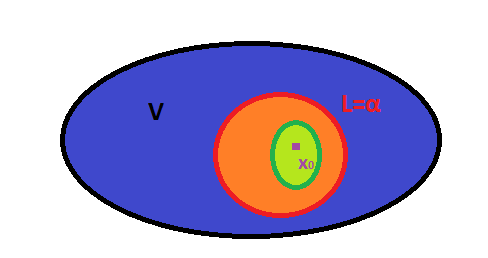
\includegraphics[scale=0.7]{lyapunov.png}
\end{figure}
\section{Instability of fixed points to autonomous ODE by Lyapunovs method}
\begin{theorem}
If $\exists$ a neighbourhood $U$ of $0$ and $V:\Omega\subset \R^n\to\R$, $0\in\Omega$, such that $V$ and $V'$ are positive definite on $U\cap\Omega\backslash\{0\}$. Then the equilibrium $0$ is completely unstable, i.e. $0$ is a repeller.
\end{theorem}
\begin{proof}
Suppose $0$ is not a repeller. Then there exists a neighbourhood $\Omega_0$ such that $\varphi(t,x_0)$ stays in $U\cap\Omega_0\backslash\{0\}$ for some $x_0\in U\cap\Omega_0\backslash\{0\}$. Then $V(\varphi(t,x_0))\geq V(x_0)>0$ for all $t\geq 0$. Let $\alpha = \text{inf}\{V'(x) : x\in U\cap\Omega_0,\, V(x)\geq V(x_0)\}>0$. Then
\begin{equation*}
V(\varphi(t,x_0)) = V(x_0) + \int_0^t V'(\varphi(s,x_0))\id s \geq V(x_0) + \alpha t.
\end{equation*}
Since $\varphi(t,x_0)$ remains in $U\cap\Omega_0\backslash\{0\}\forall t\geq 0$, $V(\varphi(t,x_0))$ is bounded for $t\geq 0$. This gives us that for $t$ sufficiently large we obtain a contradiction from the above inequality.
\end{proof}
\section{Bendixson's negative criterion}
\begin{theorem}
Consider the system
\begin{equation*}
\left\{ \begin{array}{l}
x' = f(x,y)\\
y'=g(x,y).\end{array}\right.
\end{equation*}
If $\frac{\partial f}{\partial x}+\frac{\partial g}{\partial y}$ is of the same sign in a simple-connected  domain $D$ in $\R^2$, then there are no periodic orbits on $D$.
\end{theorem}
\begin{proof}
Suppose there is a periodic orbit $C=\{x(t),y(t)\}_{0\leq t\leq T}$. Green's theorem gives 
\begin{equation*}
\begin{split}
\int\int_D \left( \frac{\partial f}{\partial x} + \frac{\partial g}{\partial y}\right) &= \oint_C -g(x,y)\id x + f(x,y)\id y = \\
& = \int_0^T \left[ -g(x(t),y(t))x'(t) + f(x(t),y(t))y'(t)\right]\id t = 0.
\end{split}
\end{equation*}
But $\frac{\partial f}{\partial x} + \frac{\partial g}{\partial y}$ is of the same sign, thus
\begin{equation*}
\int\int_D \left( \frac{\partial f}{\partial x} + \frac{\partial g}{\partial y} \right)
\end{equation*}
is either positive or negative. This is a contradiction.
\end{proof}
\end{document}